\section{Design Overview}
A fixed-function hardware as shown in Fig. \ref{figure:fixed_func_hw}, computes the L1D-cache set index based on the address bits of the memory reference. The design seeks to randomize the mapping from addresses to sets in the cache.  The hash employed is different for different addresses, as the hashing scheme involves using a swizzle of certain bits from the tag. The hash obtained after the application of the hashing scheme to the address is XOR'ed with the original index bits to generate the new cache set index. This ensures a many-to-many mapping from the original index to the index generated after applying the hashing scheme. 

\subsection{Single static hash scheme}
The hashing scheme involves swizzling of certain bits from the original tag and set index bits. The hash obtained after the application of the hashing scheme to the address is XOR'ed with the original set index bits to generate the new cache set index. This ensures a many-to-many mapping from the original index to the index generated after applying the hashing scheme. Since a single static hash scheme is used for all addresses across all the processes, we assume that the adversary can eventually figure out the hashing scheme, i.e. the ordering and bit positions obtained after swizzling. However, it does not leak any information about the victim's memory references since the final hash used for XOR'ing is computed from the victim's address which is unknown to the adversary.

\begin{figure*}
  \center{\includegraphics[width=\textwidth]
    {figures/FixedFunctionHW.pdf}}
  \caption{Fixed function hardware for computing set index}
  \label{figure:fixed_func_hw}
\end{figure*}

\subsection{Multiple static hash schemes}
In order to provide more security, we can add more hashing schemes in hardware and use(assign?) them at page granularity which is described in detail in later sections(Section No?). The hardware implements multiple hash schemes, one of which is chosen using the lower bits of the page number. With this approach, the adversary has to learn multiple schemes. Additionally, he has no knowledge of the scheme used by the address referenced by the victim which adds more entropy.

\subsection{Multiple changing hash schemes}
Instead of using statically determined hash schemes, we can provide more security by using a different hash scheme at different points of time for the same page. This can be achieved by maintaining a lookup table where each entry stores the current hash scheme and the count of cachelines using this scheme. We recycle the hash scheme for an entry once all the blocks from the pages mapped to this entry have been evicted from the L1D cache. The duration for which one or more blocks from the page are resident in the cache is refereed to as the \textit{lifetime of page in the cache}. We leverage the shorter lifetimes of pages in the L1D cache to give us a periodic change in the hashing scheme used to index into the cache. The changing hash schemes force the attacker to periodically learn the hash scheme stored in the entry of interest of the lookup table.

\subsubsection{Hash lifetimes: Variation with entries}
The duration for which a particular hash scheme is assigned to the entry in the lookup table is called the hash lifetime. Fig. \ref{figure:Hash_lifetime} shows the hash lifetimes variations with different number of lookup table entries. We observe that as we increase the number of entries in the lookup table, the percentage of hash entries with longer lifetimes reduce for most of the applications. This is because fewer pages get mapped to the same entry which enables faster recycling of hash schemes. Applications like <TODO: blah blah> see an increase in the percentage of hash entries with longer lifetimes because pages with longer lifetimes in the cache are getting mapped to different entries in the table, thus increasing hash lifetimes.
\begin{figure*}
  \center{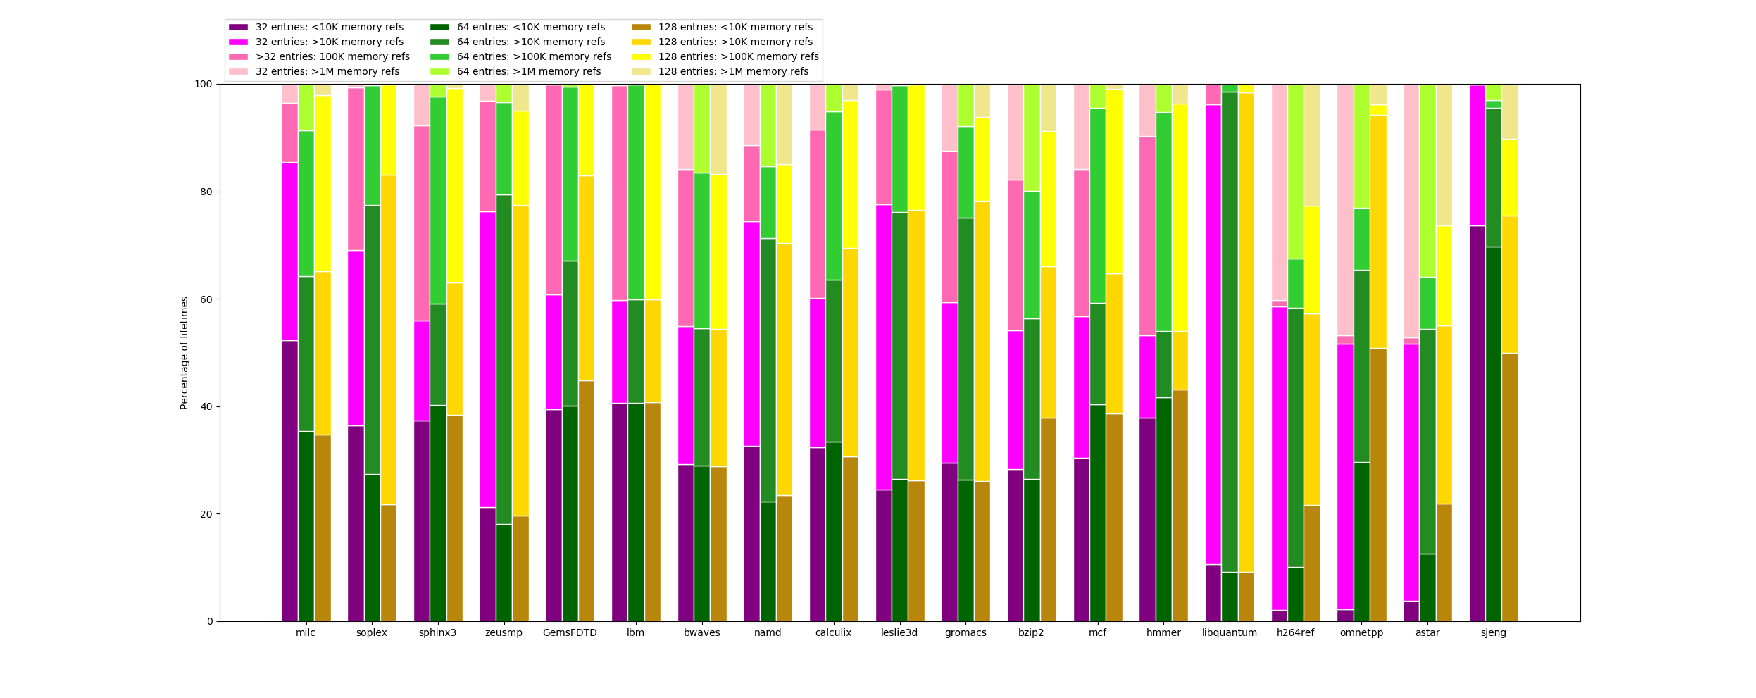
\includegraphics[width=\textwidth]
    {figures/HashLifetimes.pdf}}
  \caption{Hash lifetime variations with different number of lookup table entries}
  \label{figure:Hash_lifetime}
\end{figure*}

\subsubsection{Tolerating table lookup latency}
The table lookup can be done in parallel with the address generation, hence hiding the table lookup latency incurred with the changing hash schemes design. The address generation step entails adding the base address to the address offset. We can use the base address to index into the table and read the corresponding hash scheme and the scheme from the next entry. Once the complete address is known after address generation, we can select the true hash scheme out of the two selected before and use that to compute the set index bits. 

\subsection{Cache Design Used}
The design used here is the recently proposed VC-DSR virtual cache design \cite{}. The primary design philosophy behind this cache is to cache data indexed by an address from a primary or a leading virtual page, where the leading virtual page refers to the page that is cached first, and any synonymous access is remapped to the corresponding address from the leading virtual page.  This design inherently keeps track of the virtual pages currently present in the cache, facilitating the maintenance of hashing schemes while a virtual page is alive in the cache, and their subsequent recycling upon their exit from the cache. Additionally, the use of virtual cache allows us to hide the latency associated with the lookup of the table containing the hashing schemes by overlapping the lookup of the table with the process of generating the effective address. 

\subsection{Issues with Virtually Indexed Physically Tagged Caches}
For a virtually indexed physically tagged cache, application of such a scheme becomes more complicated. This is because synonymous addresses would get hashed differently, because bits in the virtual page number are used to index the table containing the hashing scheme to be used. These bits would be different for synonymous addresses, resulting in them using different hashing schemes. The other option would be to use bits in the physical page number to index the table containing the hashing schemes, however this would defeat the purpose of using a virtually indexed and physically tagged cache, because we would have to wait for the virtual to physical translation to complete, before we could generate the cache set index. If the same hashing scheme was applied to all sets, then the scheme would involve using bits from the physical tag, again involving waiting for the virtual to physical translation to complete. 

\subsection{Issues with Physically Indexed Physically Tagged Caches}
With a PIPT cache, the selection and application of a hash scheme can only occur after address translation. This introduces latenccy on the critical path which might be intolerable along with the address translation latency.
introduced by the table lookup. 


\subsection{Issues with present scheme(not one-to-one and increased tag size)}
The mapping from original index to the index generated after applying the hashing scheme is many-to-many. Therefore, the original tag bits alone would not suffice to uniquely identify the addresses that get mapped to the particular set. This would entail having to use larger tags in the L1 cache. In effect, because of the many-to-many mapping, our tag size increases to the size of a tag in a fully associative cache. However, the tag comparison is still to be performed only amongst the tags present in the particular set of interest. Our design allows any cacheline to reside in any of the cache locations like in a fully associative cache.  

